\chapter{Bentuk Energi dan Perubahannya}\label{ch:g9:energy-conversions}

\omterm{def:g5:everyday-energy:energy}{Energi} telah mengalir menembus buku ini seperti sungai di bawah sebuah
kota --- terlihat sekilas di setiap sudut, tetapi belum pernah
dipetakan seluruhnya. Saatnya telah tiba. Setiap bentuknya mendapat
namanya, salah satunya mendapat rumus besar kedua tahun ini, dan di
atas semuanya bertakhta hukum pembukuan yang paling perkasa di dalam
ilmu pengetahuan: totalnya tidak pernah berubah. Sama sekali.

\section{Bentuknya, dihimpun}

\begin{definition}[Bentuk energi]\label{def:g9:energy-conversions:forms}
Bentuk \omterm{def:g5:everyday-energy:energy}{energinya}, yang disajikan secara resmi:
\emph{\omterm{prop:g9:kinetic-energy-safety:formula}{energi kinetik}} --- jatah geraknya, $\frac12 m v^2$;
\emph{energi potensial}\index{energi potensial} --- yang tersimpan
oleh kedudukan atau susunan (yang terangkat, yang teregang, yang
termampatkan); \emph{\omterm{def:g5:everyday-energy:energy}{energi} termal} --- goyangan \omterm{def:g7:states-of-matter:molecule}{molekul} yang tidak
tertib yang diukur \omterm{def:g3:temperature-thermometers:temperature}{suhu}; \emph{\omterm{def:g5:everyday-energy:energy}{energi} kimia} --- yang tersimpan di
dalam susunan materi: makanan, bahan bakar, \omterm{def:g3:first-electric-circuit:battery}{baterai}; \emph{\omterm{def:g5:everyday-energy:energy}{energi}
listrik} --- yang dapat diantarkan arus yang berarak; \emph{\omterm{def:g5:everyday-energy:energy}{energi}
radiasi} --- yang dibawa \omterm{def:g1:light-and-shadows:source}{cahaya} itu sendiri, bentuk pengiriman sinar
matahari; dan \emph{\omterm{def:g5:everyday-energy:energy}{energi} nuklir} --- yang terkunci di dalam inti
atomnya, simpanan terdalam yang pernah dibuka manusia.
\end{definition}

\begin{proposition}[Energi potensial gravitasi]\label{prop:g9:energy-conversions:ep}
Mengangkat sebuah \omterm{def:g3:measuring-mass:mass}{massa} $m$ (dalam \unit{kg}) setinggi $h$ (dalam
\unit{m}) melawan $g$ milik \omterm{def:g9:gravitation:gravitation}{gravitasi} menyimpan di dalamnya \omterm{def:g9:energy-conversions:forms}{energi
potensial}
\[
E_p = m \times g \times h
\]
\omterm{def:g9:kinetic-energy-safety:joule}{joule} --- yang dapat dipulihkan sepenuhnya pada perjalanan turunnya.
Kapak yang terangkat, ayunan yang ditarik ke belakang, danau gunungnya:
semuanya menyimpan $m g h$ di rekeningnya. (Inilah rumus yang dipinjam
poster keselamatan jalannya --- kini resmi menjadi milikmu.)
\end{proposition}

\begin{example}[Pertukaran besarnya: $E_p$ lawan $E_k$]\label{ex:g9:energy-conversions:trade}
Jatuhkan sebutir bola dari tinggi $h$: selagi ia jatuh, rekeningnya
berpindah, \omterm{def:g9:kinetic-energy-safety:joule}{joule} demi \omterm{def:g9:kinetic-energy-safety:joule}{joule}, dari potensial ke kinetik. Di tanahnya,
seluruh $m g h$ telah menjadi $\frac12 m v^2$ --- samakan keduanya dan
\omterm{def:g3:measuring-mass:mass}{massanya} pun saling meniadakan:
\[
v = \sqrt{2 g h},
\]
akar kuadrat tahun ini memperoleh nafkahnya. Dari \qty{20}{m}:
$v = \sqrt{2 \times 9.8 \times 20} \approx \qty{20}{m/s}$ ---
tujuh puluh kilometer tiap \omterm{ex:g2:measuring-time:clock}{jam}, berapa pun \omterm{def:g3:measuring-mass:mass}{massanya}. Bandulnya
memainkan pertukarannya ke dua arah selamanya (dikurangi sebuah
bisikan kepada \omterm{def:g2:air-around-us:air}{udaranya}); pemain papan luncur di dalam pipa
setengahnya demikian pula: tinggi menjadi \omterm{def:g7:motion-average-speed:formula}{kelajuan} menjadi tinggi,
dengan kedua rumusnya mengoperkan satu jumlah bolak-balik.
\end{example}

\begin{omfigure}
\begin{tikzpicture}[scale=0.8]
  \draw[very thick, omExo]
    (0.4,3.4) .. controls (2.2,0.2) and (4.2,0.2) .. (6.0,3.0)
    .. controls (7.0,4.6) and (8.4,4.6) .. (9.6,3.2);
  \fill[omDef] (0.4,3.4) circle (0.16);
  \fill[omDef] (3.2,0.62) circle (0.16);
  \fill[omDef] (7.2,4.15) circle (0.16);
  \node[above, font=\footnotesize, align=center] at (0.9,3.6)
    {seluruhnya $E_p$,\\tanpa kelajuan};
  \node[below, font=\footnotesize, align=center] at (3.2,0.4)
    {seluruhnya $E_k$:\\tercepat di sini};
  \node[above, font=\footnotesize, align=center] at (7.2,4.35)
    {menukar kembali:\\lambat di puncaknya};
\end{tikzpicture}

{\small Pembukuan rol koasternya: tinggi yang dibelanjakan membeli
\omterm{def:g7:motion-average-speed:formula}{kelajuan}, \omterm{def:g7:motion-average-speed:formula}{kelajuan} yang dibelanjakan membeli tingginya kembali --- satu
jumlah, dua rekening, dan totalnya menunggangi tanpa berubah (kecuali
kikisan gesekan yang diam-diam).}
\end{omfigure}

\section{Hukum yang besar}

\begin{proposition}[Kekekalan energi]\label{prop:g9:energy-conversions:conservation}
Pada setiap proses yang pernah diperiksa --- tumbukan dan kimia, mesin
dan badai, \omterm{def:g4:solar-system:star}{bintang} dan sel --- \omterm{def:g5:everyday-energy:energy}{energi} berganti bentuk dan berganti
pemilik, tetapi \emph{totalnya} kekal dengan tepat: tidak ada yang
diciptakan, tidak ada yang dimusnahkan, dan setiap \omterm{def:g9:kinetic-energy-safety:joule}{joulenya}
dipertanggungjawabkan. Inilah hukum pembukuan yang terdalam di dalam
fisika: ia memensiunkan mesin abadi pada bab masa kecilnya, ia
memeriksa setiap rantai di dalam buku ini, dan tidak ada percobaan
dalam tiga abad yang menangkapnya berbuat kesalahan. (Mengapa alam
menaati hukum ini dengan begitu setia adalah pertanyaan yang mendalam
dengan jawaban yang indah --- salah satu permata tahun-tahun perguruan
tinggi.)
\end{proposition}

\begin{method}[Memeriksa proses apa pun]\label{met:g9:energy-conversions:audit}
Pembukuan semesta milik sang fisikawan:
\begin{enumerate}
  \item pagari sistemnya --- apa yang berada di dalam pemeriksaannya;
  \item sebutkan rekening \omterm{def:g5:everyday-energy:energy}{energinya} sebelumnya: tiap bentuknya, tiap
        simpanannya;
  \item sebutkan semuanya sesudahnya --- termasuk, selalu, uang kecil
        termalnya: kehangatan gesekannya, bisikan \omterm{def:g3:sound-around-us:sound}{bunyinya};
  \item seimbangkan pembukuannya: totalnya harus berpadanan. Sebuah
        kekurangan berarti ada bentuk yang tidak terhitung ---
        lihatlah lagi kebocorannya; biasanya ia hangat.
\end{enumerate}
\end{method}

\begin{example}[Pemeriksaan, dikerjakan]\label{ex:g9:energy-conversions:audits}
Mobil yang mengerem: rekening kinetiknya dikosongkan, rekening termal
pada cakramnya dikreditkan sepenuhnya --- pensiun, bukan pemusnahan.
Bola yang memantul lalu mati perlahan: tiap pantulannya mengikis
kinetiknya menjadi kehangatan bola dan lantainya; jawaban masa
kecilnya, kini dapat diperiksa. Sarapanmu yang bersepeda menanjak:
simpanan kimianya turun, rekening potensialnya naik ($m g h$ milik
dirimu dan sepedanya), dengan jatah termalnya diradiasikan --- ototnya
berjalan hangat. Setiap misteri pada bab \omterm{def:g5:everyday-energy:energy}{energi} yang awal tertutup di
bawah ketiga lajur yang sama.
\end{example}

\section{Efisiensi}

\begin{definition}[Efisiensi]\label{def:g9:energy-conversions:efficiency}
\emph{Efisiensi}\index{efisiensi} sebuah pengubah adalah bagian \omterm{def:g5:everyday-energy:energy}{energi}
masukannya yang diantarkan dalam bentuk yang diinginkan:
\[
\text{efisiensi} =
\frac{\text{energi berguna yang keluar}}{\text{energi total yang masuk}},
\]
sebuah bilangan di antara $0$ dan $1$ (atau persentasenya). Sisanya
tidak dimusnahkan --- kekekalannya melarang --- melainkan lolos dalam
bentuk yang tidak diinginkan, yang hampir selalu berupa kehangatan.
\end{definition}

\begin{example}[Rapor]\label{ex:g9:energy-conversions:reportcards}
\omterm{def:g3:first-electric-circuit:bulb}{Bohlam} leluhur yang berpijar: lima persen \omterm{def:g1:light-and-shadows:source}{cahaya}, sembilan puluh lima
persen kehangatan --- sebuah pemanas yang punya hobi. Penerusnya yang
sezaman: tiga puluh persen lebih, sisanya tetap kehangatan. Sebuah
mesin mobil: kira-kira sepertiga menjadi gerak yang berguna, dua
pertiganya keluar lewat radiator dan knalpotnya. Sebuah \omterm{ex:g6:circuits-and-safety:motor}{motor} listrik:
di atas sembilan puluh. \omterm{def:g9:alternator:alternator}{Alternator} yang besar: dekat sembilan puluh
sembilan --- pengubah terbaik milik peradaban. Tidak ada pengubah yang
jujur yang mencapai seratus: sedikit kebocoran menjadi kehangatan
adalah komisi semesta milik alam.
\end{example}

\begin{omfigure}
\begin{tikzpicture}[scale=0.8]
  \draw[omDef, fill=omDef, fill opacity=0.4]
    (0.3,1.2) rectangle (4.2,2.6);
  \node[font=\small] at (2.25,1.9) {masukan: \qty{100}{J}};
  \draw[omMeth, fill=omMeth, fill opacity=0.4]
    (7.4,2.0) rectangle (11.2,2.9);
  \node[font=\footnotesize] at (9.3,2.45)
    {berguna: \qty{35}{J}};
  \draw[omThm, fill=omThm, fill opacity=0.35]
    (7.4,0.6) rectangle (11.2,1.75);
  \node[font=\footnotesize] at (9.3,1.17)
    {kehangatan: \qty{65}{J}};
  \draw[-Stealth, very thick] (4.3,2.25) -- (7.3,2.5);
  \draw[-Stealth, very thick] (4.3,1.55) -- (7.3,1.2);
  \node[above, font=\small] at (5.8,2.65) {pengubah};
\end{tikzpicture}

{\small Sebuah diagram \omterm{def:g9:energy-conversions:efficiency}{efisiensi}: seratus \omterm{def:g9:kinetic-energy-safety:joule}{joule} masuk, tiga puluh lima
diantarkan sebagaimana diinginkan, enam puluh lima bocor sebagai
kehangatan --- dan tidak satu \omterm{def:g9:kinetic-energy-safety:joule}{joule} pun hilang dari jumlahnya.}
\end{omfigure}

\begin{omfigure}
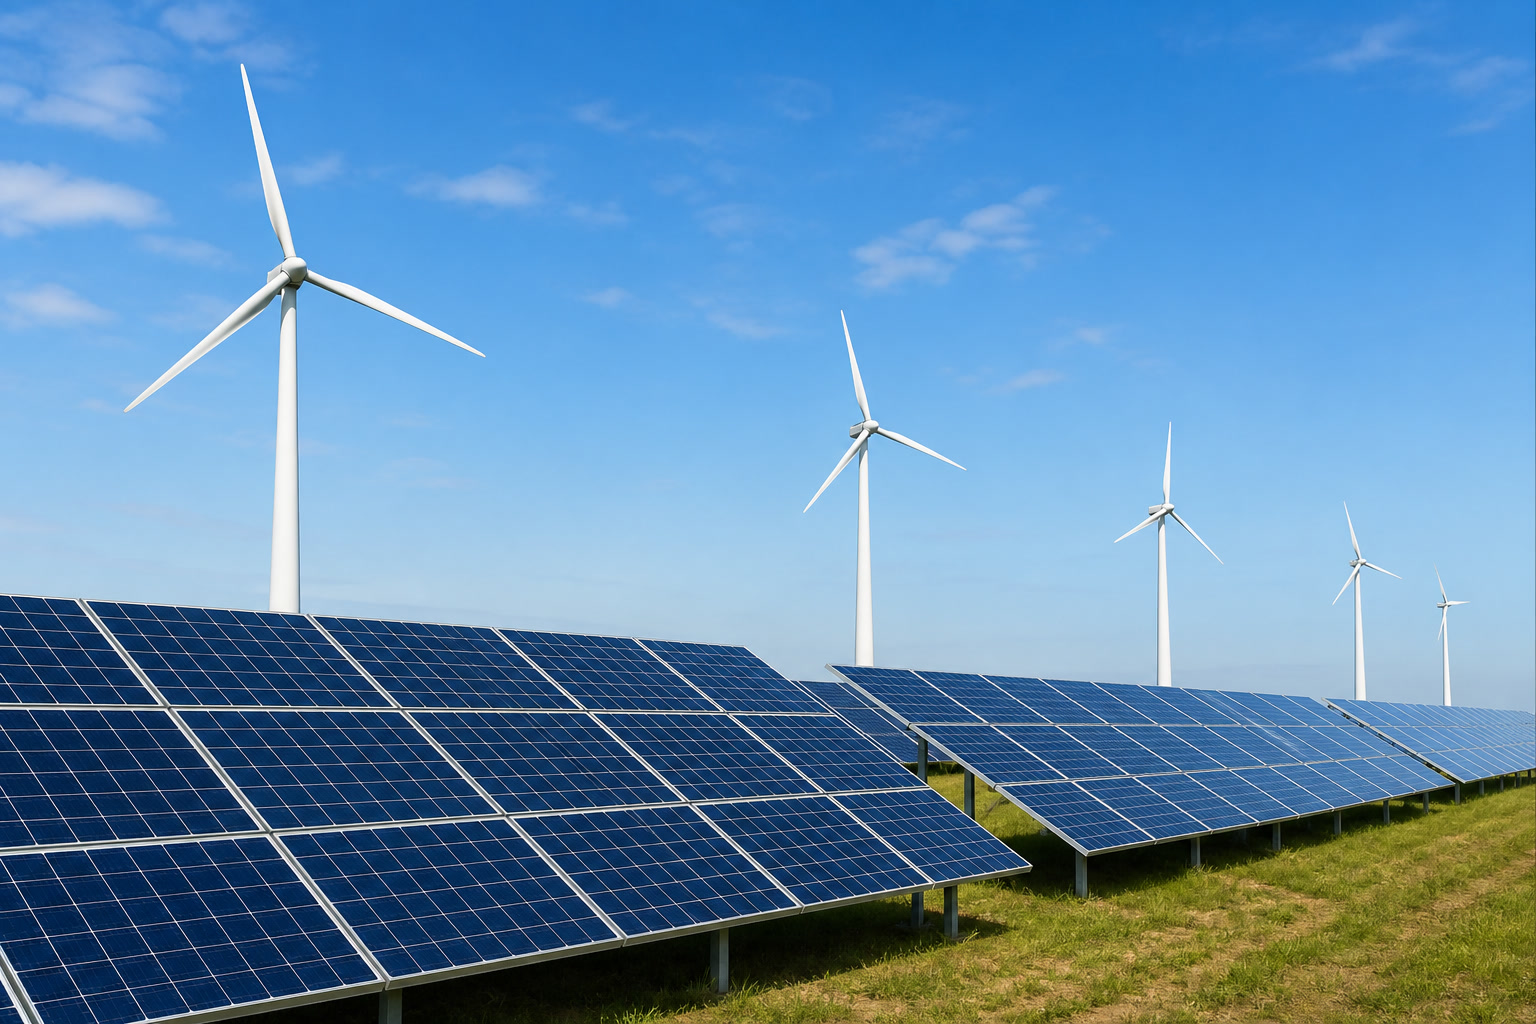
\includegraphics[width=0.55\linewidth]{images/book1/ai/g9-energy-solar-wind.jpg}

{\small Dua pengubah di satu ladang: \omterm{def:g1:light-and-shadows:source}{cahaya} matahari menjadi \omterm{def:g5:everyday-energy:energy}{energi} listrik di dalam panelnya, \omterm{def:g2:air-around-us:air}{udara} yang bergerak menjadi \omterm{def:g5:everyday-energy:energy}{energi} listrik di dalam turbinnya.}
\end{omfigure}

\begin{remark}[Apa arti sesungguhnya ``menghemat energi'']\label{rem:g9:energy-conversions:saving}
Kalau kekekalannya menjaga setiap \omterm{def:g9:kinetic-energy-safety:joule}{joule}, mengapa siapa pun harus
``menghemat \omterm{def:g5:everyday-energy:energy}{energi}''? Karena hukumnya menjaga \emph{jumlahnya}, bukan
\emph{kegunaannya}. Simpanan yang terpusat --- bahan bakar, muatan,
tinggi --- dapat dibelanjakan menjadi kehangatan yang tersebar tipis
menembus dunianya, dan kehangatan yang tersebar, walaupun setiap
\omterm{def:g9:kinetic-energy-safety:joule}{joulenya} selamat, tidak dapat lagi menggerakkan cerek atau kereta:
sungainya sudah mengalir turun. Persoalan \omterm{def:g5:everyday-energy:energy}{energi} peradaban bukanlah
kekurangan \omterm{def:g9:kinetic-energy-safety:joule}{joule} --- Matahari menghujani kita dengan ribuan kali
kebutuhan kita --- melainkan pengelolaan \omterm{def:g9:kinetic-energy-safety:joule}{joule} yang \emph{berguna}.
Gagasan itu, kalau dibuat cermat, adalah salah satu kisah yang paling
termasyhur di dalam fisika; ia menanti pada tahun-tahun perguruan
tinggi dengan namanya yang termasyhur.
\end{remark}

\section{Latihan}

\begin{exercise}[$\star$]\label{exo:g9:energy-conversions:1}
Sebutkan ketujuh bentuk pada katalognya, masing-masing dengan satu
contoh rumah tangga.
\end{exercise}

\begin{exercise}[$\star$]\label{exo:g9:energy-conversions:2}
Hitunglah $E_p$: sebuah ember \qty{2}{kg} yang dinaikkan \qty{10}{m};
seorang pendaki \qty{60}{kg} di puncak pendakian \qty{500}{m}.
\end{exercise}

\begin{exercise}[$\star$]\label{exo:g9:energy-conversions:3}
Nyatakan hukum kekekalannya, dan apa yang dilakukannya terhadap mesin
abadi pada bab masa kecilmu.
\end{exercise}

\begin{exercise}[$\star$]\label{exo:g9:energy-conversions:4}
Periksalah bandulnya sepanjang satu ayunan: rekeningnya di puncaknya,
di dasarnya, dan pergeseran lambatnya secara keseluruhan --- ke mana?
\end{exercise}

\begin{exercise}[$\star$]\label{exo:g9:energy-conversions:5}
Pakailah $v = \sqrt{2 g h}$: \omterm{def:g7:motion-average-speed:formula}{kelajuan} cebur dari papan loncat
\qty{5}{m} --- lalu mengapa \omterm{def:g3:measuring-mass:mass}{massa} peloncatnya tidak pernah masuk.
\end{exercise}

\begin{exercise}[$\star$]\label{exo:g9:energy-conversions:6}
Batasilah \omterm{def:g9:energy-conversions:efficiency}{efisiensi}. Sebuah \omterm{ex:g6:circuits-and-safety:motor}{motor} mengambil \qty{200}{J} lalu
mengantarkan \qty{170}{J} gerak: berapa \omterm{def:g9:energy-conversions:efficiency}{efisiensinya}, dan apa nasib
sisanya?
\end{exercise}

\begin{exercise}[$\star$]\label{exo:g9:energy-conversions:7}
Mengapa \omterm{def:g3:first-electric-circuit:bulb}{bohlam} leluhurnya cukup adil disebut ``sebuah pemanas yang
punya hobi''? Berikan kedua persentasenya.
\end{exercise}

\begin{exercise}[$\star$]\label{exo:g9:energy-conversions:8}
Tuliskan rantai perubahan yang penuh milik pendakian pengendara
sepedanya --- dari sarapan sampai puncak --- sambil menyebut tiap
bentuknya dan tiap kebocorannya.
\end{exercise}

\begin{exercise}[$\star\star$]\label{exo:g9:energy-conversions:9}
Pembukuan bendungannya: \qty{1000}{kg} air jatuh \qty{50}{m}
menembus turbinnya. Hitunglah $E_p$ yang diantarkan; pada pengubahan
sembilan puluh persen, berapa \omterm{def:g5:everyday-energy:energy}{energi} listriknya tiap ton --- lalu
berapa ton tiap sekon yang diperlukan untuk keluaran
\qty{4.4e6}{W}.
\end{exercise}

\begin{exercise}[$\star\star$]\label{exo:g9:energy-conversions:10}
Sebutir bola \qty{0.5}{kg} yang dijatuhkan dari \qty{2}{m} melenting
kembali sampai \qty{1.2}{m}. Periksalah pantulannya: \omterm{def:g5:everyday-energy:energy}{energinya} sebelum
dan sesudahnya, ukuran kikisannya dan tujuannya --- lalu tinggi
lentingan yang sesudahnya tidak ada pemeriksaan yang akan menemukan
sisa \omterm{prop:g9:kinetic-energy-safety:formula}{energi kinetik} atau potensial.
\end{exercise}

\begin{exercise}[$\star\star$]\label{exo:g9:energy-conversions:11}
``Liftnya mengubah \omterm{def:g5:everyday-energy:energy}{energi} listrik menjadi \omterm{def:g9:energy-conversions:forms}{energi potensial} pada
\omterm{def:g9:energy-conversions:efficiency}{efisiensi} sembilan puluh persen.'' Hitunglah \omterm{def:g5:everyday-energy:energy}{energi} listrik untuk
menaikkan sebuah kabin \qty{500}{kg} setinggi \qty{30}{m} --- lalu
rukunkan sepuluh persen tambahannya dengan hukum kekekalannya.
\end{exercise}

\begin{exercise}[$\star\star\star$]\label{exo:g9:energy-conversions:12}
Pemain papan luncur di pipa setengahnya mulai dari keadaan diam di
bibir kiri, pada tinggi \qty{4}{m}. Ramalkan \omterm{def:g7:motion-average-speed:formula}{kelajuan}
penyeberangannya di dasarnya, tinggi yang dicapainya di kanan ---
secara ideal dan secara sungguhan --- lalu sketsakan nasib jangka
panjang geraknya dan \omterm{def:g5:everyday-energy:energy}{energinya}. Lalu jelaskan, dengan
\cref{rem:g9:energy-conversions:saving}, mengapa dorongan apa pun di
bibirnya tidak akan pernah dapat dipulihkan sepenuhnya: apa yang
diperoleh pembukuan dunianya, dan apa yang hilang tak terpulihkan dari
pemain papan luncurnya?
\end{exercise}

\section{Soal: Penugasan Taman Hiburan}

\begin{problem}[{Soal akhir pekan --- taman hiburannya mempekerjakan
seorang penasihat fisika; rol koaster, menara, dan pembukuan yang tidak
dapat berdusta}]\label{pb:g9:energy-conversions:1}
Wahana baru tamannya harus lulus pemeriksaan energimu sebelum hari
pembukaannya. Ambillah $g = \qty{9.8}{N/kg}$; abaikan gesekannya
sampai ia menolak diabaikan.

\medskip\noindent\textbf{Bagian I --- Terjunan Besarnya.}
Sebuah rangkaian koaster \qty{2000}{kg} diderek ke puncak \qty{45}{m}
lalu dilepaskan dari keadaan diam.
\begin{enumerate}
  \item Berapa $E_p$ rangkaiannya di puncaknya?
  \item Berapa \omterm{def:g7:motion-average-speed:formula}{kelajuan} idealnya di dasar terjunannya, menurut rumus
        yang meniadakan \omterm{def:g3:measuring-mass:mass}{massanya} --- dalam \unit{m/s} dan
        \unit{km/h}?
  \item Para perancangnya menambahkan bukit kedua setinggi \qty{50}{m}
        tepat sesudah terjunannya. Tolaklah dengan pembukuannya ---
        lalu nyatakan bukit kedua tertinggi yang dapat dipuncaki
        rangkaian yang ideal.
  \item \omterm{def:g7:motion-average-speed:formula}{Kelajuan} dasar yang terukur \qty{28}{m/s}, bukan yang
        idealnya. Hitunglah kedua \omterm{prop:g9:kinetic-energy-safety:formula}{energi kinetiknya} lalu bebankan
        selisihnya pada rekening yang sepatutnya.
\end{enumerate}

\medskip\noindent\textbf{Bagian II --- Dereknya dan
tagihannya.}
\begin{enumerate}[resume]
  \item Dereknya mengangkat rangkaiannya ke puncaknya dalam
        \qty{60}{s}. Pada \omterm{def:g9:energy-conversions:efficiency}{efisiensi} yang sempurna, berapa \omterm{def:g9:electric-power-energy:power}{dayanya}?
  \item Derek yang sesungguhnya menarik \qty{20}{kW}. Berapa
        \omterm{def:g9:energy-conversions:efficiency}{efisiensinya}?
  \item Tiap wahananya berjalan tiap empat menit, sepuluh \omterm{ex:g2:measuring-time:clock}{jam} tiap
        hari. Berapa \omterm{def:g5:everyday-energy:energy}{energi} harian dereknya dalam \omterm{def:g9:electric-power-energy:kwh}{kilowatt-jam} (derek
        yang sesungguhnya, hitunglah angkatannya), dan berapa biayanya
        pada $0.25$ tiap \omterm{def:g6:measurement-in-science:measuring}{satuan}?
  \item Seorang perancang mengusulkan memulihkan \omterm{def:g5:everyday-energy:energy}{energi} kedatangan
        rangkaiannya dengan sebuah rem-pembangkit yang memberi makan
        jaringannya --- ``wahananya membayar dirinya sendiri!''
        Periksalah mimpinya: bagian berapa yang secara masuk akal
        dapat kembali, dan hukum yang mana yang melarang lingkaran
        penuhnya?
\end{enumerate}

\medskip\noindent\textbf{Bagian III --- Menara jatuh bebasnya
dan laporannya.}
Menara \qty{60}{m}-nya menjatuhkan sebuah gondola \qty{500}{kg} ke
dalam rem magnetik pada \qty{10}{m}.
\begin{enumerate}[resume]
  \item Berapa \omterm{def:g7:motion-average-speed:formula}{kelajuannya} ketika memasuki daerah remnya (jatuh ideal
        \qty{50}{m})?
  \item Berapa \omterm{def:g5:everyday-energy:energy}{energi} yang harus dipensiunkan remnya, dan ke mana
        induksinya mengirimnya. (Remnya adalah sepupu bab
        \omterm{def:g9:alternator:alternator}{alternatornya} --- pusaran arus induksi yang memanaskan
        logamnya.)
  \item Penumpangnya menjerit bahwa mereka ``tanpa \omterm{def:g4:weight-and-mass:weight}{berat}'' selama
        jatuhnya. Dari gagasan teman-yang-sama-jatuh pada bab
        \omterm{def:g9:gravitation:gravitation}{gravitasinya}, berilah putusan atas pengakuannya dalam satu
        kalimat.
  \item Tandatangani laporan penugasannya: tiga kalimat ---
        pertukaran yang menjadi hidup koasternya, hukum yang ditaati
        setiap wahananya, dan rekening yang diam-diam menagih pajak
        kepada semuanya.
\end{enumerate}
\end{problem}
